\documentclass[../TGMAFFIRO]{subfiles}

\begin{document}
	

% TODO: write about what's to expect about this chapter: explain what is to come in this chapter and how will it be developed, following the next steps.
% 	*The first part will relax riguourous assumptions 
% in order to build an intuition of the brownian motion as the limit of a random walk
% 	* The second part will get into he details of L2 spaces and the connection with
% the BM and the rest of the work
% 	* The third and final part will prove some important components of the brownian motion
% and the geometric brownian motion as an example of this.


% 1) Link
In chapter one we posed the question about the theoretical value of a financial call option that starts today. Specifically, we want to answer the following question: what is today's value for a derivative that pays $\max\{S_T-K, 0\}$ at maturity? Note that, at time $T$, the payoff of the option is a function of $S_T$, since all else is given. Consequently, preceding the valuation of any option we must first take into account the dynamics of the asset we are referring to, i.e., we must come up with a model for $S_t$ for all $t \in [0,\infty)$.\\

% 2) Focus
In the following chapter, we aim to attain a model that explains the random changes of financial assets. More precisely, what is needed is to describe the ``noise'' of an asset over time by virtue of stochastic processes.\\

% 3) Overview
We begin by motivating the need for such processes in a mathematically-informal way; we continue laying the mathematical foundations for what is the final process to model the \textit{noise}; finally, we conclude the chapter by proving remarkable properties about the latter.

\section{Random Walks}
Suppose that two players (A and B) toss an even coin $n$ times, one toss for every unit of time\footnote{Note that this unit of time can be one second, one day, 5 minutes, etc.}. Whenever tails comes up, A will pay B \$1. On the contrary, A will receive \$1 from B. Suppose further that we decide to model how much did A won (or lost) after $n$ tosses. To do so, we define the following:

\begin{definition}\label{srwalk}
	Let $\{X_j\}_{j\geq0}$ be a set of independent and identically distributed (i.i.d.) random variables for which $\Pm(X_i = \pm 1) = \frac{1}{2}$; $i \geq 1$. Define $M_0 = 0$ and
	\begin{equation}
		M_n := \sum_{k=1}^n X_k \ \forall \ n \in \mathbb{N}.
	\end{equation}
	The process $\{M_d\}_{d\geq 0}$ is known as a \textbf{symmetric random walk}
\end{definition}

%%% Symmetric random walk figure %%%
\begin{figure}
	\label{fig:symmetric_random_walk}
	\centering
	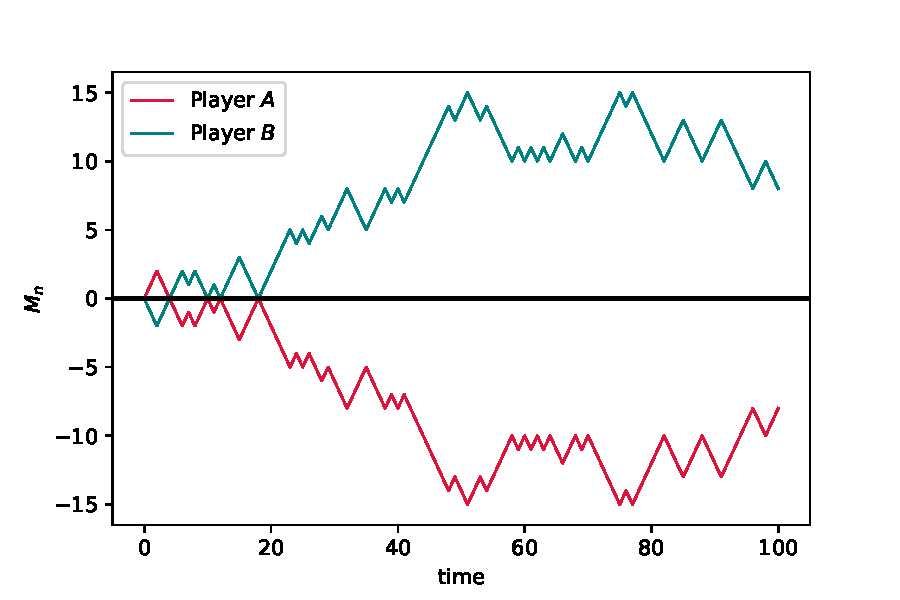
\includegraphics[width=0.9\textwidth]{images/symmetric_random_walk}
	\caption{Path of a Symmetric Random Walk}
\end{figure}

\begin{proposition}\label{prop:expectation_srw}
	The expected value of a symmetric random walk is 0.
\end{proposition}

\begin{proof}
	Let $n \in \mathbb{N}$ then,
	\begin{align*}
	\mathbb{E}(M_n) &= \mathbb{E}\left[X_0 + \sum_{i=1}^d X_i\right]\\
				    &= 0 + n  \left( 1 \cdot \frac{1}{2} + (-1) \cdot \frac{1}{2}\right).
	\end{align*}
\end{proof}

Proposition \ref{prop:expectation_srw} shows that the definition of a symmetric random walk (\ref{srwalk}) captures what we intended to model. From the outset, both players start with with \$0 and, as the game progresses, whichever amount A wins, B looses it. The type of games, in which the amount player $A$ wins, player $B$ losses it are called \textbf{zero-sum games}.\\

After a large number of times played we expect to break even. Nobody would win or loose once played a large number of times\footnote{In fact, according to Law of Large Number, we would expect to break even after a number so large that it approaches to infinity.}\\

A symmetric random walk also happens to be known as a fair-game. This is because what one would expect to win at any given future point in time is dependent on the amount that one has today. In other words, if both of the players start with a P\&L of \$0, then they would not expect, after a large amount of games\footnote{Mathematically speaking, the expectation of the game is zero in the sense that, as the number of games tends to infinity, the average P\&L for any of the players turn to zero} to earn any more money than what they started with: \$0.\\

To see why, consider the following proposition

\begin{proposition}
	The simple random walk is a martingale for $k < \ell$
\end{proposition}

\begin{proof}
	\begin{align*}
				\mathbb{E}[M_\ell|\salgF_k] &= \mathbb{E}[(M_\ell - M_k) + M_k | \salgF_k] \\
				&= \mathbb{E}[(M_\ell - M_k) | \salgF_k] + \mathbb{E}[M_k | \salgF_k] \\
				&= \mathbb{E}[M_\ell - M_k] + M_k\\
				&= M_k
	\end{align*}
\end{proof}

No matter the point in time in the future that we refer to, the value that one would expect to have in the future the one that we have today. As a consequence, the only \textit{useful} information we have today about the future value of the game, is the one we have today.

\section{Scaled Random Walk}
The simple random walk can altered such that between any two units of time the process takes $n$ steps.

\begin{definition}
	We define the \textbf{scaled random walk} $W^n(t)$ as the following transformation of the simple random walk:
	\[W^n(t) := \frac{1}{\sqrt{n}}M_{nt}\]
\end{definition}

\begin{remark}
	The scaled random walk has the following properties:
	\begin{itemize}
		\item The increments are independent: \[\left(W^n(t_{i+1}) - W^n(t_{i})\right) \perp \left(W^n(t_{j+1}) - W^n(t_{j})\right) \ \forall \ i \neq j \ i, j \geq 1\]
		\item For $s < t$, and $ns$,  $nt$ $\in \mathbb{W}$, 
		\begin{itemize}
			\item $\mathbb{E}[W^n(t_{i}) - W^n(t_{j})] = 0$; and
			\item $\mathbb{V}[W^n(t_{i}) - W^n(t_{j})] = t - s$.
		\end{itemize}
		\item The Scaled random walk is a martingale: for all $k < \ell$
		\[\mathbb{E}[W^n(\ell) | \salgF_k] = W^n(k)\].
	\end{itemize}
\end{remark}

One complication arises in modeling a financial asset, that of choosing the partition between any two units of time. Consider fig.\ref{fig:scaled_random_walk}, it shows sample paths for different partitions of time. As the number of partition increases, the number of possible path increases too. Conversely, if there is only one partition, the process will reach either 1 or -1. With this in mind, the question of whether there exists a \textit{correct} partition for a particular asset may seem partial and confined.\\

%%% Scaled Random Walk figure %%%
\begin{figure}[h]
	\label{fig:scaled_random_walk}
	\centering
	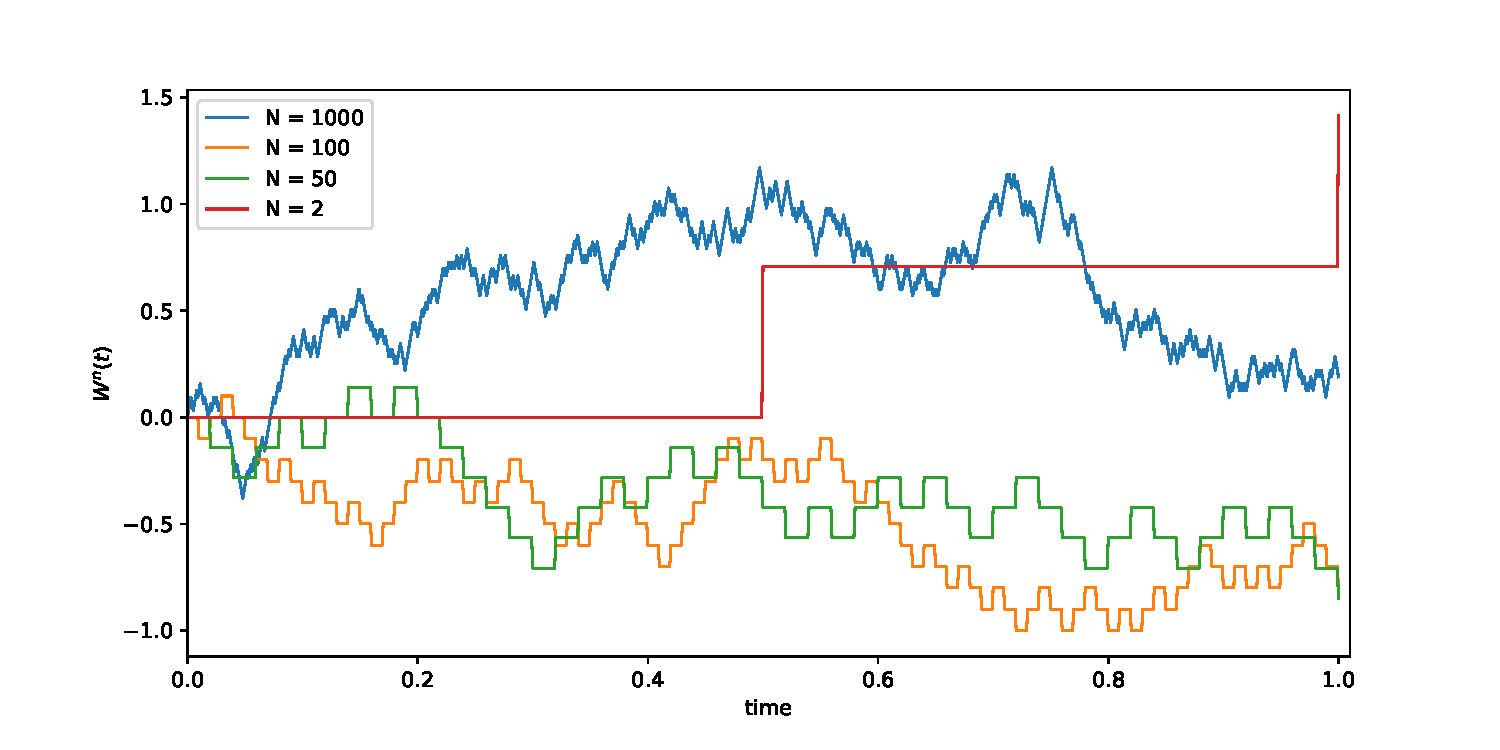
\includegraphics[width=0.9\textwidth]{images/scaled_random_walk}
	\caption{Scaled Random Walk}
\end{figure}


To further develop this theory we will start assuming that the market moves in continuous time. This, as we will later see, allow us to use more sophisticated methods to work with the process while generalizing this to any market we desire. This assumptions leads to an important theorem that will help us keep building the model for the financial asset.

\begin{theorem}\label{th:convergence_rw}
	Let $t \geq 0$. As $n \to \infty$, the distribution of the scaled random walk $W^n(t)$ converges to a normal distribution with mean $0$ and variance $t$.
\end{theorem}

\begin{proof}
	We will show that the moment generating function for a symmetric random walk tends to the moment generation function of a normal with $\mu = 0$ and $\sigma^2 = t$.\\
	
	Denote $\varphi_n(u)$ and $\varphi(u)$ the moment generating functions of the symmetric random walk and the normal distribution respectively. We will then show that $\varphi_n(u) \to \varphi(u)$. Where $\varphi_n(u) = \left(\frac{1}{2}e^{\frac{u}{\sqrt{n}}} + \frac{1}{2}e^{-\frac{u}{\sqrt{n}}}\right)^{nt}$ and $\varphi(u) = e^{\frac{1}{2}u^2t}$ (Refer to appendix \ref{proof:mgf_srm} and \ref{proof:mgf_nd} for the derivation of both moment generating functions).\\
	
	Since,
	\begin{equation*}
		\varphi_n(u) = \left(\frac{1}{2}e^{\frac{u}{\sqrt{n}}} + \frac{1}{2}e^{-\frac{u}{\sqrt{n}}}\right)^{nt}.
	\end{equation*}
	Then,
	\begin{equation}
		\ln\varphi_n(u) = nt\cdot\ln\left(\frac{1}{2}e^{\frac{u}{\sqrt{n}}} + \frac{1}{2}e^{-\frac{u}{\sqrt{n}}}\right).
	\end{equation}
	Let $x = \frac{1}{\sqrt{n}}$, and take the limit as $n$ tends to infinity,
	\begin{align*}
		\lim_{n\to\infty}\ln\varphi_n(u) &= \ln\lim_{n\to\infty}\varphi_n(u) \tag*{($\varphi_n$ is cont. at $n > 0$) }\\
		&= \lim_{x\to 0} \frac{t\ln\left(\frac{1}{2}e^{ux}+ \frac{1}{2}e^{-ux}\right)}{x^2}
		\intertext{Applying l'H\^opital's rule}
		&= \frac{t}{2}\lim_{x\to 0}\frac{\frac{u}{2}e^{ux} - \frac{u}{2}e^{-ux}}{x}
		\intertext{Applying l'H\^opital's rule again}
		&= \frac{t}{2}\lim_{x\to 0}\left(\frac{u^2}{2}e^{ux} + \frac{u^2}{2}e^{-ux} \right).
	\end{align*}
	
	We conclude, $\lim_{n\to\infty}\varphi_n(u) = e^{\frac{1}{2}u^2t}$.
\end{proof}

Theorem \ref{th:convergence_rw} shows the distribution that follows at every time $t$ if we assume that the market moves continuously. The process that emerges from this assumption is paramount in what follows. In fact, this process has a name of its own, which we will denote the \textbf{Brownian motion}.\\

In what follows of this chapter, we formalize the \textbf{Brownian motion}
\section{$L_2$ Spaces}
\begin{definition}
	let $V$ a linear space, we define a \textbf{norm} over v as the function $\norm{\cdot}: v \in V \to \RNums$ such that, for every $v\in V$, $\alpha \in \RNums$
	\begin{enumerate}
		\item $\norm{v}\geq 0$;
		\item $\norm{v} = 0 \iff v = 0$;
		\item $\norm{\alpha x} = |\alpha| \norm{x}$; and
		\item $\norm{v + w} = \norm{v} + \norm{w}$.
	\end{enumerate}
\end{definition}	
We say that $(V, \norm{\cdot})$ is a complete normed spaced (or a Banach space) i, for $\{v_n\}_{n\geq 0}$, and $\{v_m\}_{m\geq 0}$; $\norm{v_n - v_m} \to 0$ as $n, m \to \infty$. The sequence $\{\norm{v_m, v_n}_{n,m \geq 0}\}$ is known as a \textbf{Cauchy sequence}. This last fact imposes the existence of $v\in V$ such that $\lim_{n\to\infty} v_n = v$.

\begin{definition}
Let $\ProbSpace$ be a measurable space, we define the $L_2$ space ($L_2\ProbSpace$) as the family of random variables such that
	\begin{equation}
		\norm{X}_2:= \left(\E[|X|^2] \right)^{1/2} < \infty
	\end{equation}
	
\end{definition}

%TODO: Proof!
It can be shown that if $X$, $Y$ are two random variables such that $\Pm(X=Y) = 1$, then the linear normed space $(L_2, \norm{\cdot}_2)$ is a Banach space.

\section{Brownian Motion}
\begin{definition}\label{def:brownian_motion}
	A \textbf{Brownian Motion} with parameter $\sigma^2$ is a stochastic process $\{W_t \in \RNums:t\geq 0\}$ that satisfies the following properties:
	\begin{itemize}
		\item $W_0 = 0$
		\item The trajectories are continuous
		\item The process has independent increments
		\item $\forall \ 0 \leq s \leq t \Longrightarrow (W_t - W_s) \sim N(0, \sigma^2(s - t)$
	\end{itemize}
\end{definition}

\begin{remark}
	A Brownian Motion with $\sigma^2 = 1$ is known as a Standard Brownian Motion.
\end{remark}

The Brownian Motion is a first desirable result since it allow us to work in continuous time. Furthermore, it allow us to measure a probability at every $t\geq 0$ with tools already known for continuous random variables. 

%%% Arithmetic Brownian Motion Image %%%
\begin{figure}[h]
	\centering
	\label{fig:Brownian_Motion}
	\includegraphics[width=0.9\textwidth]{images/bm}
	\caption{Sample Paths of a Brownian Motion}
\end{figure}

Although it is computationally impossible to properly simulate a Brownian Motion, it can be approximated via the scaled random walk for big $n$. Figure \ref{fig:Brownian_Motion} shows this idea approximating a brownian motion with $n=9000$. In pursuance of pricing a European call option, we will see that it is possible to arrive at a closed form solution for these types of option. Nevertheless, more complex products may or may not have a closed form solution\\

To further develop the properties of the Brownian Motion, let us define the following:
\begin{definition}\label{def:quadratic_variation}
	Let $f$ be a real-valued function defined over $[0, T]$. Consider a partition $\Pi= \{t_i\}_{i=0}^{n}$ over $[0, T]$ where $t_0 = 0$, $t_n = T$, and $||\Pi|| = \max_j\{t_{j+1} - t_j\}$. We define the \textbf{Quadratic Variation} of $f$ up to time $T$ as
	\[
		[f, f]_T := \lim_{||\Pi|| \to 0} \sum_{t=0}^{n-1}\left[f(t_{j+1}) - f(t_{j})\right]^2
	\]
\end{definition}


The quadratic variation for a function $f$ represents the amount of total quadratic oscillation inside $D = [0,T]$. It can be shown (see \aycite{shreve}) that for $f \in C^1(D)$, $[f,f]_T = 0$.\\
	
Asking how much does $W(t)$ oscillates between $D$ posses the question of whether $W(t) \in C^1(D)$. The answer is no, since the Brownian Motion is a continuous, nowhere-differentiable function. A consequence of this last remark is the following.

\begin{theorem}\label{th:quadratic_brownian_motion}
	Let $W(t)$ be a Standard Brownian Motion, then $[W, W]_T = T \ \forall \ T \geq 0$ almost surely.
\end{theorem}

\begin{proof}
	Let $\Pi = \{t_j\}_{j=0}^n$ be a partition of $[0, T]$. Define the sample quadratic variation corresponding to this partition to be
	
	\[
		Q_{\Pi} = \sum_{j=0}^{n-1}(W_{t_{j+1}} - W_{t_{j}})^2
	\]
	
	To show that $[W, W]_T = T$, is equivalent to show that, as $n\to\infty$, $\mathbb{E}[Q_\Pi] = T$ and $\mathbb{V}(Q_\Pi) = 0$ almost surely.\\
	
	First note that, by definition of the Standard Brownian Motion,
	\begin{equation}\label{eq:exp_change_bm}
		\mathbb{E}[(W_{t_{j+1}} - W_{t_{j}})^2] = \mathbb{V}[W_{t_{j+1}} - W_{t_{j}}] = t_{j+1} - t_{j}
	\end{equation}
	
	\begin{equation}\label{eq:var_change_bm}
		\mathbb{V}([W_{t_{j+1}} - W_{t_{j}}]^2) = 2(t_{j+1} - t_{j})^2
	\end{equation}
	
	Refer to appendix \ref{proof:var_change_bm} for a derivation of eq. \ref{eq:var_change_bm}.\\
	
	Consider now
	\begin{align*}
		\mathbb{E}[Q_\Pi] &= \mathbb{E}[\sum_{j=0}^{n-1}(W_{t_{j+1}} - W_{t_{j})}^2] \\
		&= \sum_{j=0}^{n-1}\mathbb{E}[(W_{t_{j+1}} - W_{t_{j}})^2] \\
		&= \sum_{j=0}^{n-1}(t_{j+1} - t_{j}) \\
		&= T
	\end{align*}
	
	Now,
	\begin{align*}
		\mathbb{V}(Q_T) &= \mathbb{V}(\sum_{j=0}^{n-1}(W_{t_{j+1}} - W_{t_{j}})^2) \shortintertext{By independence,}
		&=  \sum_{j=0}^{n-1}\mathbb{V}((W_{t_{j+1}} - W_{t_{j}})^2)\\
		&= \sum_{j=0}^{n-1} 2(t_{j+1} - t_{j})^2 \\
		&\leq 2 \sum_{j=0}^{n-1}||\Pi||\cdot (t_{j+1} - t_{j}) \numberthis
	\end{align*}
	
	Finally, note that
	
	\begin{equation}
		\lim_{||\Pi||\to 0} 2 \sum_{j=0}^{n-1}||\Pi||\cdot (t_{j+1} - t_{j}) = \lim_{||\Pi||\to 0} 2 ||\Pi|| T = 0
	\end{equation}
	$\therefore \lim_{||\Pi||\to 0} Q_\Pi = T$ almost surely.
\end{proof}

We state theorem \ref{th:quadratic_brownian_motion} informally by writing
\begin{equation}
	dW^2 = dt
\end{equation}

Two final consequences of \ref{th:quadratic_brownian_motion} are the following
\begin{equation}\label{eq:wt_0}
	\lim_{||\Pi||\to 0} \sum_{j=0}^{n-1}(W_{t_{j+1}} - W_{t_{j}})(t_{j+1} - t_{j}) = 0
\end{equation}

\begin{equation}\label{eq:w2_0}
	\lim_{||\Pi||\to 0} \sum_{j=0}^{n-1}(t_{j+1} - t_{j})^2 = 0
\end{equation}

Equations \ref{eq:wt_0} and \ref{eq:w2_0} are informally expressed as $dW_tdt = 0$ and $dt^2 = 0$

\end{document}